\documentclass{article}
\usepackage[utf8]{inputenc}
\usepackage{hyperref}
\usepackage{url}
\usepackage{mathtools}
\usepackage{amsmath}
\usepackage{graphicx}
\usepackage{wrapfig}
\usepackage{algorithm}
\usepackage{algpseudocode}
\usepackage{subcaption}
\usepackage[svgnames]{xcolor}
\usepackage{listings}
\usepackage[left=2.5cm, right=2.5cm, top=1.5cm, bottom=2cm]{geometry}
\setcounter{section}{-1}


\title{
\textbf{Algorithmics for Data Mining: Deliverable 2\\} \Large{
    Handwitten images classificator}}
\author{Oriol Borrell\\
\textit{\small FIB - UPC Student} \\
\textit{\small Barcelona, Spain} \\
\textit{\texttt{\href{mailto:oriol.borrell.roig@est.fib.upc.edu}
{\small oriol.borrell.roig@est.fib.upc.edu}}}}
\date{\today}

\begin{document}
\maketitle

\section{Abstract}
\textit{
In this project we have trained a model \footnote{Github repository of the project: \url{https://github.com/oriolborrellroig/ADM-Deliveries/tree/master/SecondDelivery}} in order to classify handwritten images within a given categories. In the last essay we focused on on the preprocessing, we thought for a easy solution to deal with outliers, and finally we built a KNN model in order to classify the images, obtaining a accuracy of 0.7 (with two categories). In this delivery we will increase the number of categories. We also will search for a model that obtains a better accuracy than a KNN.
}

\section{Introduction}
\label{Modeling}
In order to train our models, we will need to prepossess the new data. We used in the preprocessing the exact same steps explained n the first delivery. The only change is that now we are using 5 categories, containing around 5000 drawings each. Take into account that once discarded the outliers, the number of drawings will be reduced. 

\section{k-Nearest Neighbors (KNN)} 
\label{KNN}
Once we had the data ready we splitted our data in into train and test data (75\%-25\%). Afterwords, we tried to find the $k$ that give us a better accuracy. We tried all the odd values from $1$ to $30$. Table \ref{tab:knn_results} shows the obtained values:

\begin{table}[H]
    \centering
    \begin{tabular}{|l|l|l|}
        \hline
        \textbf{k} & \textbf{accuracy}  \\
        \hline
        1 & 18.59\% \\
        \hline
        3 & 19.34\% \\
        \hline
        5 & 20.38\% \\
        \hline
        7 & 25.58\% \\
        \hline
        9 & 26.49\% \\
        \hline
        11 & 27.94\% \\
        \hline
        13 & 27.53\% \\
        \hline
        15 & 28.03\% \\
        \hline
        17 & 31.32\% \\
        \hline
        19 & 32.86\% \\
        \hline
        21 & 33.43\% \\
        \hline
        23 & 33.52\% \\
        \hline
        25 & 33.89\% \\
        \hline
        27 & 33.43\% \\
        \hline
        \textbf{29} & \textbf{34.27\%} \\
        \hline
    \end{tabular}
    \caption{Accuracy obtained respect $k$}
    \label{tab:knn_results}
\end{table}

As the higher accuracy was obtained with $k=29$, we used this value to build our model. We re-trained the classifier and tried to predict the drawings that we reserved for validation. We got an accuracy of 0.3427. As it happened in the previous delivery, we obtain a better prediction that we would obtain flipping a coin (0.2). However, this accuracy is not enough. After a bit of research, I found that Convolutional Neural Networks (CNN) are very good for predicting images. In the following section we will try to increase the accuracy with a CNN.

\section{Convolutional Neural Networks (CNN)}
\label{CNN}

A Convolutional Neural Network (CNN) is a specific type of artificial neural network that has some hidden layers called convolutional layers, where the transformation is made in this layer is a convolutional operation. CNNs is widely used to do image recognition, image classifications, objects detections, faces recognition etc., that's the reason I choosed this algorithm.

The model type that was used was Sequential. It allows you to build a model layer by layer. In our model we will use the following type of layers:

\begin{itemize}
    \item \textbf{Conv2D:} This layer creates a convolution kernel that is convolved with the layer input to produce a tensor of outputs.
    \item \textbf{MaxPool2D:} Takes the maximum value of the kernel to reduce the number of parameters.
    \item \textbf{SpatialDropout2D:} We randomly set entire kernel to 0. So we will drop them, in order to prevent for overfiting.
    \item \textbf{Flatten:} It reduces the dimension of the data into 1 dimension.
    \item \textbf{Dropout:}It randomly turn off neurons in order to reduce overfitting.
    \item \textbf{Dense:} We take the dimension created in the flattern layer and convert it into the category to predict.
    
\end{itemize}
 
The following table shows the CNN i designed:

\begin{table}[ht]
    \centering
    \begin{tabular}{|l|ccc|}
        \hline
        \textbf{Layer(type)} & \textbf{Units} & \textbf{Filter} & \textbf{Stride} \\
        \hline
        Conv2D & 8 & 5 & 2 \\ \hline
        Conv2D & 32 & 3 & 1\\ \hline
        MaxPool2D & - & 3 & 2\\ \hline
        SpatialDropout2D & - & - & -\\ \hline

        Conv2D & 64 & 3 & 2\\ \hline
        Conv2D & 64 & 3 & 1\\ \hline
        MaxPool2D & - & 3 & 2\\ \hline
        SpatialDropout2D & - & - & -\\ \hline

        Conv2D & 128 & 1 & 1\\ \hline
        Conv2D & 128 & 1 & 1\\ \hline
        Conv2D & 128 & 1 & 1\\ \hline
        SpatialDropout2D & - & - & -\\ \hline

        Flatten & - & - & -\\ \hline
        Dropout & - & - & -\\ \hline
        Dense & 5 & - & -\\ \hline

    \end{tabular}
    \caption{Accuracy obtained respect $k$}
    \label{tab:knn_results}
\end{table}

When we built the model we tried allot of possibles parametritzations for the number of nodes in each Conv2D layer. Finaly, in the first set of layers we have 8 nodes, and 32, tn the second one two layers of 64 nodes, and in the third one three layers of 128 nodes. This are the number of nodes that made us reach the higher accuracy. Another parametrization we choosed was the kernel size, the size of the filter matrix for our convolution. We decided to create $3 \times 3$ size filter matrix, except in the first layer, that will be a $5 \times 5$ matrix, and in the last set of Conv2D layers.

We also had to define the number of \textit{epochs} (number of times we train the model with the same training/testing data) we will perform. If we set a low number of epochs our model could not be enough trained. If we set a big number of epochs, our model could be overfitted. In both cases the accuracy will decrease, so the number of epochs important.

\begin{figure}[H]
    \centering
    \begin{subfigure}{.49\textwidth}
      \centering
      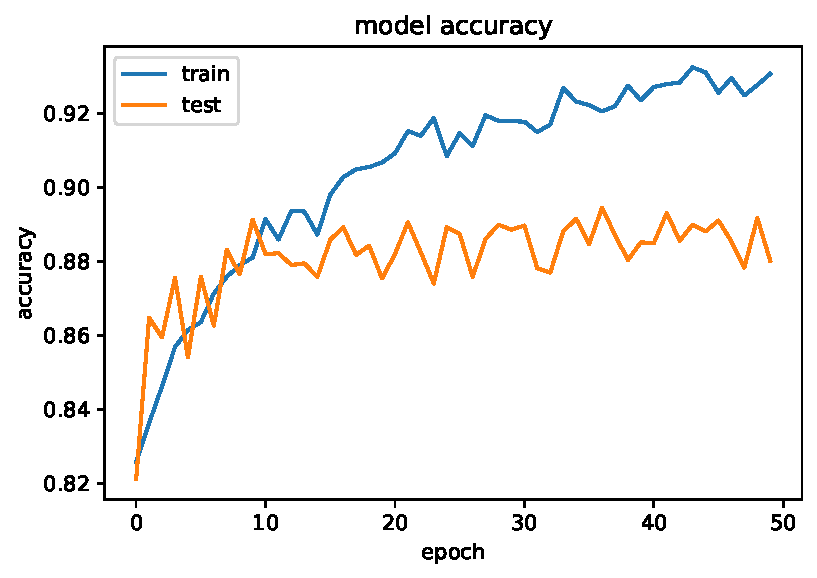
\includegraphics[width=1\textwidth]{./img/epochs_accuracy.pdf}
      \caption{Accuracy in each epoch}
      \label{fig:EpochAccuracy}
    \end{subfigure}
    \begin{subfigure}{.49\textwidth}
        \centering
        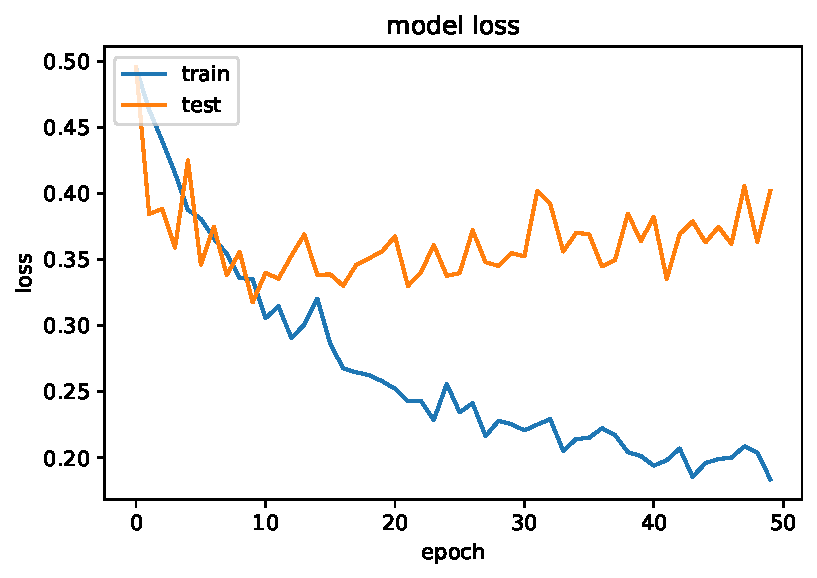
\includegraphics[width=1\textwidth]{./img/epochs_loss.pdf}
        \caption{Loss in each epoch}
        \label{fig:EpochLoss}
    \end{subfigure}
    \caption{Evaloation of epochs}
    \label{fig:EvaloationOfEpochs}
\end{figure}

So we first built the model with 50 epochs, and plotted the acuracy and lost values of each one. In Figures \ref{fig:EpochAccuracy} and \ref{fig:EpochLoss} we can clearly see that after epoch 15 we have a overfitted model, as is when in both figures the train and test lines are starting to take different directions. So we rebuilt the model with 15 epochs.

With all this parametritzations, once built the model we validated with the data saved for that purpose. We obtained an accuracy of \textbf{0.8373}. With this model we can be much more confident of our prediction in comparison to $k$-NN. We have to take into account that CNN is a neural network, and this works well with huge amount of data. So is probable that if we train the model with much more data, the accuracy will be higher.

\section{Evaluation do the results}

The results obtained with a KNN clasifier gave us an improvement comparing it with "flipping a coin" to predict the category. However, the accuracy obtained is not the one that we expected.  Comparing the two models we created, for this project we would clearly choose the CNN one. The best parametrization we found for the CNN gave us a 0.8373 of accuracy, which we conclude that is an acceptable result for this project. 

However, the important thing of this project was not only to obtain a high accuracy, but also to learn the different parts of a CNN and to detect overfitting. We also can affirm that we completed this goal of the project.

\section{Implementation}
In order to play a little with the model we built, just for fun, we drew som images using the paint application for windows operating systems. We used our model to predict the their category. The images created are the ones shown in Figure \ref{fig:PaintDrawings}:

\begin{figure}[H]
    \centering
    \begin{subfigure}{.25\textwidth}
      \centering
      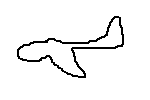
\includegraphics[width=1\textwidth]{./img/1.png}
      \caption{Aircraft1}
      \label{fig:Aircraft1}
    \end{subfigure}
    \begin{subfigure}{.25\textwidth}
        \centering
        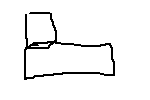
\includegraphics[width=1\textwidth]{./img/2.png}
        \caption{Aircraft Carrier}
        \label{fig:AircraftCarrier}
    \end{subfigure}
    \begin{subfigure}{.25\textwidth}
        \centering
        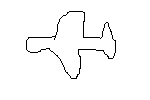
\includegraphics[width=1\textwidth]{./img/3.png}
        \caption{Aircraft2}
        \label{fig:Aircraft2}
    \end{subfigure}
    \begin{subfigure}{.25\textwidth}
        \centering
        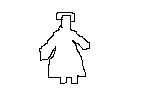
\includegraphics[width=1\textwidth]{./img/4.png}
        \caption{Angel}
        \label{fig:Angel}
    \end{subfigure}
    \begin{subfigure}{.25\textwidth}
        \centering
        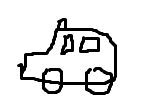
\includegraphics[width=1\textwidth]{./img/5.png}
        \caption{Ambulance}
        \label{fig:Ambulance}
    \end{subfigure}
    \begin{subfigure}{.25\textwidth}
        \centering
        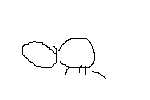
\includegraphics[width=1\textwidth]{./img/6.png}
        \caption{Ant}
        \label{fig:Ant}
    \end{subfigure}
    \caption{Paint drawnigs}
    \label{fig:PaintDrawings}
\end{figure}


The Table shows the obtained predictions. Each column represents a image (each letter refers to the letters assigned in Figure \ref{fig:PaintDrawings}). Each row represents the probability the model said of being for a certain category:

\begin{table}[ht]
    \centering
    \begin{tabular}{|l|cccccc|}
        \hline
        \textbf{Category} & \textbf{a} & \textbf{b} & \textbf{c} & \textbf{d} & \textbf{e} & \textbf{f} \\
        \hline
        Ambulance           & 0.00\% & 0.05\% & 0.12\% & 0.00\% & 100.00\% & 0.00\%   \\ \hline
        Angel               & 0.00\% & 0.00\% & 0.00\% & 99.97\% & 0.00\% & 0.00\% \\ \hline
        Aircraft carrier    & 1.49\% & 99.85\% & 12.67\% & 0.00\% & 0.00\% & 0.00\%  \\ \hline
        Airplane            & 98.51\% & 0.08\% & 84.13\% & 0.00\% & 0.00\% & 0.00\%  \\ \hline
        Ant                 & 0.00\% & 0.02\% & 3.07\% & 0.03\% & 0.00\% & 100.00\%  \\ \hline

    \end{tabular}
    \caption{Accuracy obtained respect $k$}
    \label{tab:knn_results}
\end{table}


\end{document}
